
  \documentclass{exam}

  \usepackage{units} 
  \usepackage{graphicx}
  \usepackage[fleqn]{amsmath}
  \usepackage{cancel}
  \usepackage{float}
  \usepackage{mdwlist}
  \usepackage{booktabs}
  \usepackage{cancel}
  \usepackage{polynom}
  \usepackage{caption}
  \usepackage{fullpage}
  \usepackage{xfrac}
  \usepackage{enumerate}

  \newcommand{\degree}{\ensuremath{^\circ}} 
  \everymath{\displaystyle}

  % \begin{figure}[H]
  %   \centering
  %   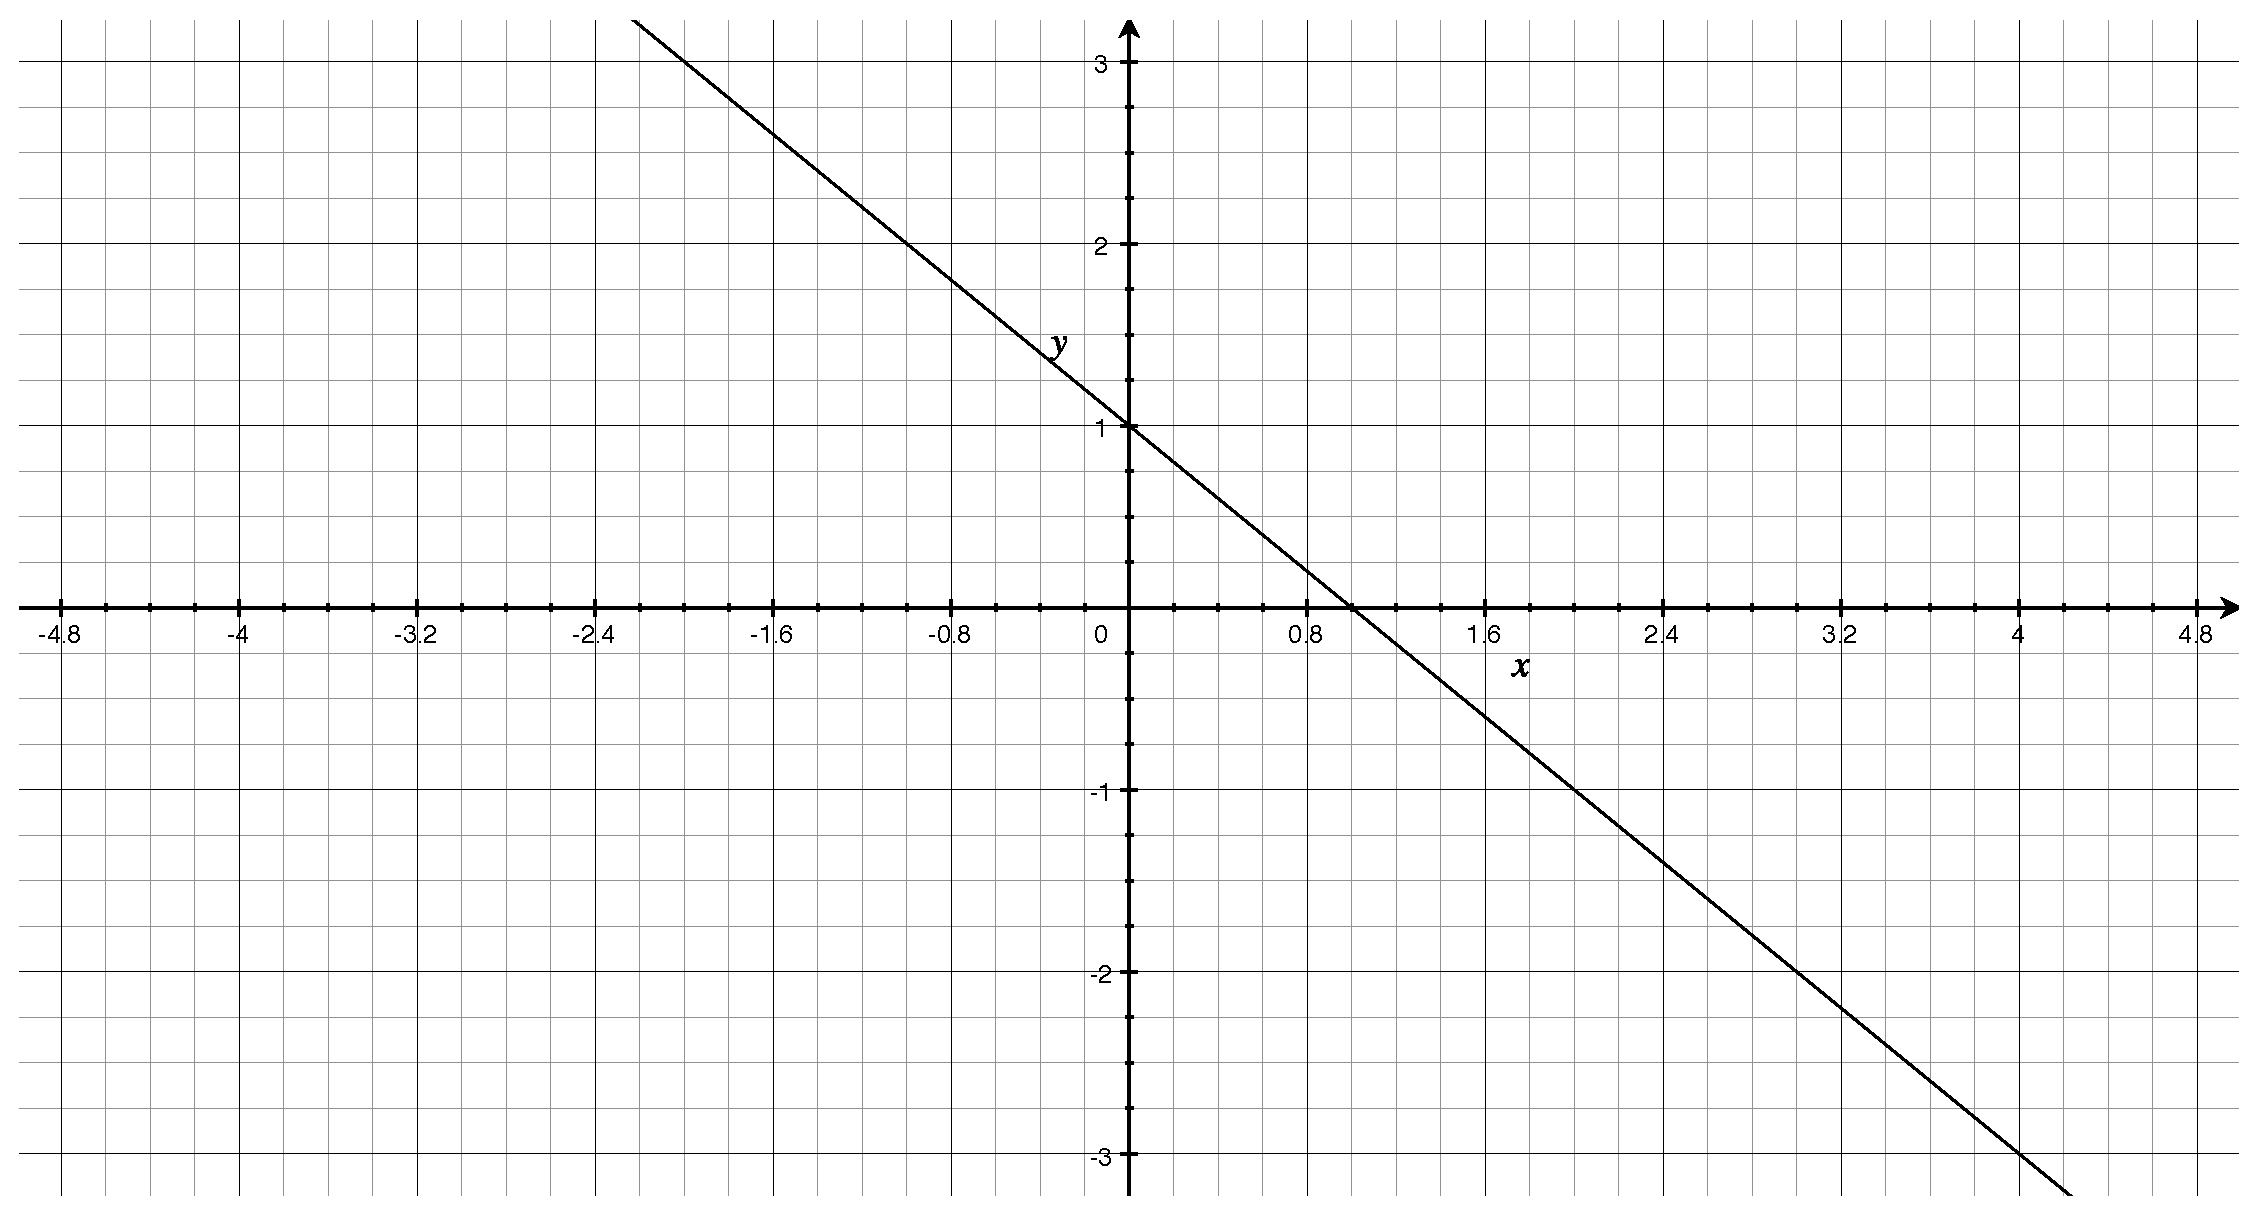
\includegraphics[scale=0.8]{problem7.eps}
  %   \caption*{Problem 7}
  % \end{figure}

  % \begin{tabular}{cc}
  %   \toprule
  %   period & amplitude \\
  %   \midrule
  %   value one & value two
  %   \bottomrule
  % \end{tabular}

  % \printanswers

  \ifprintanswers 
    \usepackage{2in1, lscape} 
  \fi

  \date{July 3, 2013}
  \author{}
  \title{Math 141 \\ Homework 17}

  \begin{document}

    \maketitle

    \section{Homework}

    Section 4.5: 

    \section{Extra Credit}
    Section 4.5: 

    \ifprintanswers
      \begin{description}
        \item[52] TO DO
      \end{description}
    \fi

    \section{Review}

    Find all the real zeros
    \begin{enumerate}
      \item $2x^3 + 5x^2 - 23x + 10 = 0$
        \ifprintanswers
          TO DO
        \fi
    \end{enumerate}

  \ifprintanswers
    \section{Section 4.5}

    \begin{description}

      \item[7]
        \begin{align*}
          3 e^x &= 10 \\
          e^x   &= \frac{10}{3} \\
          x     &= \ln \frac{10}{3} \\
                &\approx \boxed{1.20397} \\
        \end{align*}

    \end{description}

  \else
    \vspace{6 cm}
    \begin{quote}
      \begin{em}
        \ldots most legislators, politicians, lawyers, ministers, and office-holders, serve the state chiefly with their
        heads; and, as they rarely make any moral distinctions, they are as likely to serve the devil, without intending
        it, as God. A very few, as heroes, patriots, martyrs, reformers in the great sense, and men, serve the state with
        their consciences also, and so necessarily resist it for the most part; and they are commonly treated as enemies
        by it.      
      \end{em}
    \end{quote}
    \hspace{1 cm} --Henry David Thoreau
  \fi


  % chomsky:
        % The political policies that are called conservative these days would appall any genuine conservative, if there
        % were one around to be appalled. For example, the central policy of the Reagan Administration---which was
        % supposed to be conservative---was to build up a powerful state. The state grew in power more under Reagan than
        % in any peacetime period, even if you just measure it by state expenditures. The state intervention in the
        % economy vastly increased. That's what the Pentagon system is, in fact; it's the creation of a state-guaranteed
        % market and subsidy system for high-technology production.

        % The ``corporatization of America'' during the past century has been an attack on democracy—and on markets,
        % part of the shift from something resembling "capitalism" to the highly administered markets of the modern
        % state/corporate era. A current variant is called "minimizing the state," that is, transferring decision-making
        % power from the public arena to somewhere else: "to the people" in the rhetoric of power; to private tyrannies,
        % in the real world.

\end{document}

